%
% File: chap01.tex
% Author: Victor F. Brena-Medina
% Description: Introduction chapter where the biology goes.
%
\let\textcircled=\pgftextcircled
\chapter{Designing the CLB}
\label{chap:CLB_design}

\section{Overview}
\paragraph{}

This chapter provides the architecture design process of a CLB. The design and simulation setup is explained in section 2.2. The design/simulations have been done in Cadence Virtuoso. The stress induced in the silicon wafer due to copper is modeled as a function of $(r, \theta)$, as explained in section 2.3 and section 2.4. A summary of this chapter is given in section 2.5.

\section{CLB architecture: area estimation}
\paragraph{}
The architecture wireframe of the CLB used is shown in Fig 2.1.
\begin{figure}[H]
\centering
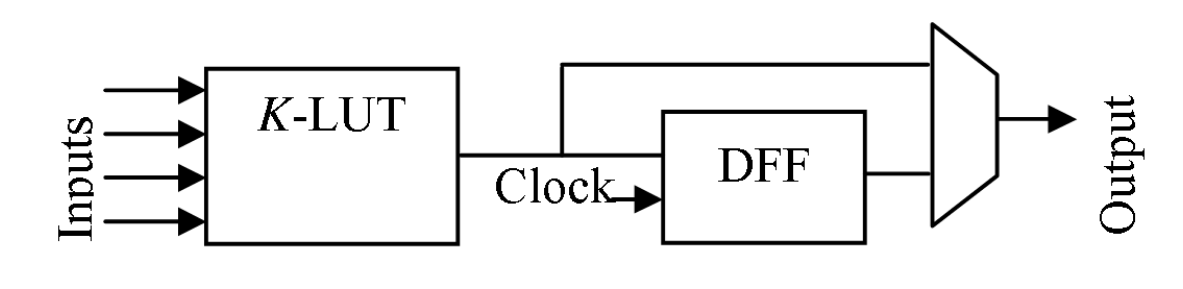
\includegraphics[width=0.7\linewidth]{CLB_wireframe.png}
\caption{CLB Architecture Wireframe}
\label{fig:Figure}
\end{figure}
 Now, we have to determine the optimum LUT size to be kept in each CLB to balance area and delay requirements for our technology. If the LUT size(K) is too small, a large number of CLBs will be needed to implement a given design which will incur a lot of routing and thus might use more area and produce a lot of delay. If K is too large, the granularity of logic will be coarse and thus even small boolean functions will take up a whole CLB. The routing area and number of CLBs will be less but the area of one CLB will be more. Thus, we need to strike a good balance for K to have reasonable granularity, area and delays. For this, we develop a model of CLB area similar to [3]. The Fig of our area model describes a tile which we use iteratively to produce the whole FPGA.

\begin{figure}[h]
\centering
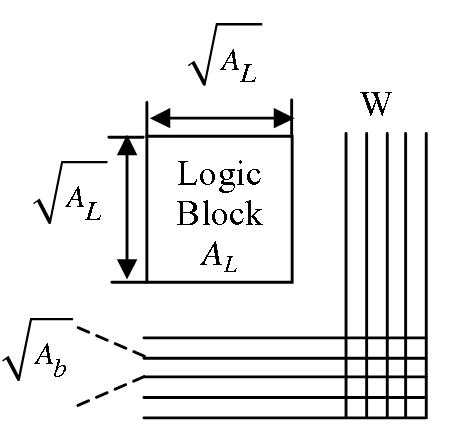
\includegraphics[width=0.3\linewidth]{area_model.png}
\caption{Area model}
\label{fig:Figure}
\end{figure}
The area of this tile can be expressed as the sum of the CLB area(or Logic area) and the area of the routing tracks as expressed below.
\begin{equation}
A_{Tile}^K = A_L^K + A_R^K
\end{equation}
Now, the logic area can be expressed as the sum of (i) $2^K$ bits to store the K-input truth table, (ii) area of one Flip-Flop, (iii) area of input crossbar, (iv) area of output crossbar and the area of configuration bits. We note that the configuration bits will be of the order of O($K.\log_{2}K$+$\log_{2}W$) which is negligible to O($2^K$) of truth table bits and thus can be ignored in an approximation. The input and output crossbars can be assumed of the same height as that of the LUT. Thus, we get the following approximate estimate of CLB area:
\begin{equation}
A_L^K = A_{bit}\cdot2^K + A_{FF} + \sqrt{A_{bit}}\cdot(\sqrt{A_{bit}\cdot2^K}\cdot\log_{2}{K}+\sqrt{A_{bit}\cdot2^K}\cdot\log_{2}{W_K})
\end{equation}
Now, the routing area can be expressed as the sum of 2 rectangles and a square as follows:
\begin{equation}
A_R^K = A_{bit}\cdot{W_K^2} + 2\cdot\sqrt{A_{bit}}\cdot{W_K}\cdot\sqrt{A_L^K}
\end{equation}
Adding logic and routing areas, we get the following area per tile:
\begin{equation}
A_{Tile} = {(\sqrt{A_{bit}}\cdot{W_K}+\sqrt{A_L^K})}^2 + A_{bit}\cdot2^{K/2}\cdot\log_{2}{(KW_K)}
\end{equation}
To find the area of the whole FPGA, we need to multiply the tile area with the number of CLBs needed in total. For that, we need an estimate of the number of CLBs required to implement a given design. The Rent-rule[6] proposes an empirical relationship b/w No. of input pins(T) and No. of logic blocks(N) given below:
\begin{equation}
T = \lambda\cdot{N^p}
\end{equation}
where $\lambda$ is a proportionality constant and p is the Rent-exponent shown to be around 0.75 for FPGA devices in [7]. [3] uses the following two equations to approximate $W_k$ and $N_k$ with $N_2$ to be $10^4$ for K=2:
\begin{equation}
\frac{N_2}{N_k} = {(\frac{K+1}{3})}^{\frac{1}{p}}
\end{equation}
\begin{equation}
W_K = \frac{K+1}{2}\cdot\frac{2}{3}\cdot\frac{1-p}{p-0.5}\cdot({(N_k)}^{p-0.5}-1)
\end{equation}
Now, the total area of the FPGA becomes $N_k$ time the area of one tile plus some extra routing area to account for two edges of the formed FPGA:
\begin{equation}
A_{Total} = A_{Tile}\cdot{N_k} + 2\cdot\sqrt{N_k}\cdot(A_{bit}\cdot{W_K^2} + \sqrt{A_{bit}\cdot{A_L^K}}\cdot{W_K})
\end{equation}
We use the shown layouts for area estimates of a Flip-Flop(168.27 um sq.) and SRAM cell(16 um sq.).
\begin{figure}[h]
\begin{subfigure}{0.6\textwidth}
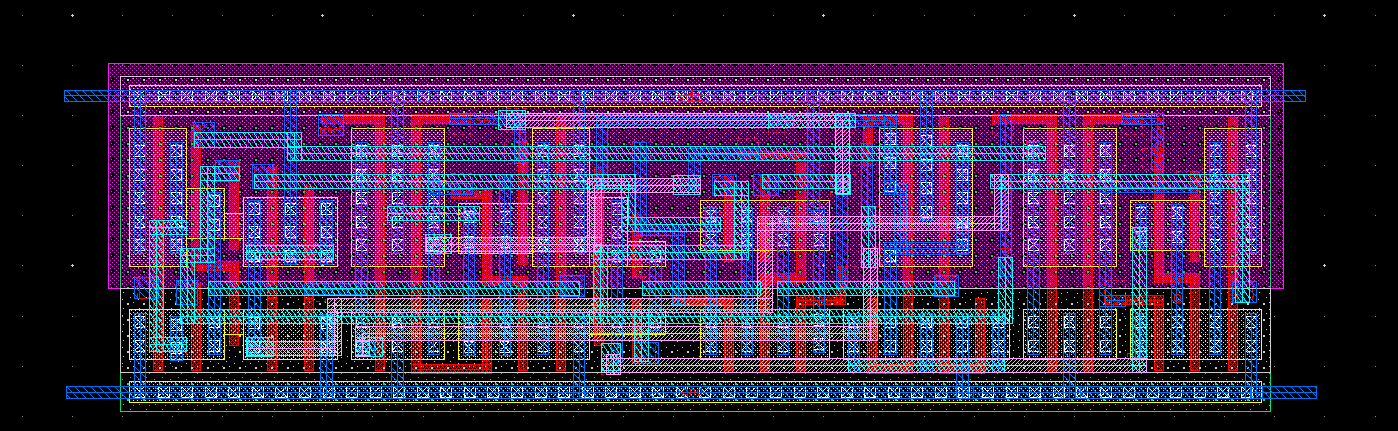
\includegraphics[width=0.9\linewidth, height = 0.35\linewidth]{DFF.png} 
\caption{Layout of DFF}
\label{fig:Figure}
\end{subfigure}
\begin{subfigure}{0.3\textwidth}
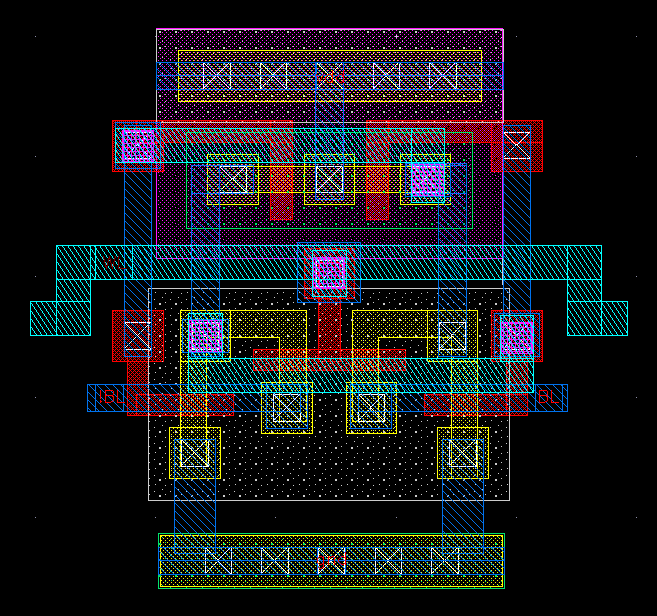
\includegraphics[width=0.9\linewidth, height = 0.8\linewidth]{SRAM.png}
\caption{Layout of SRAM cell}
\label{fig:Figure}
\end{subfigure}
\caption{Layouts for area estimates}
\label{fig:Figure}
\end{figure}
 
\begin{figure}[h]
\centering
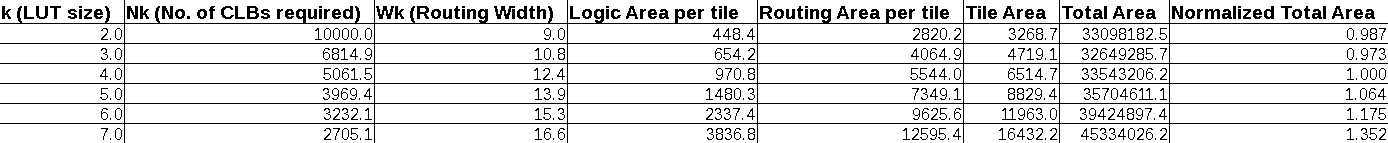
\includegraphics[width=\linewidth]{area_table.png}
\caption{Area estimates in $um^2$ for different values of k}
\label{fig:Figure}
\end{figure}

\begin{figure}[h]
\begin{subfigure}{0.5\textwidth}
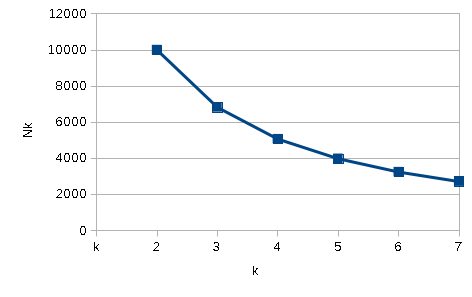
\includegraphics[scale=0.55]{k_vs_Nk.png} 
\caption{Nk vs k}
\label{fig:Figure}
\end{subfigure}
\begin{subfigure}{0.5\textwidth}
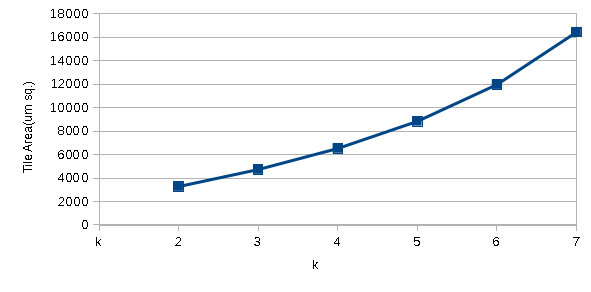
\includegraphics[scale=0.55]{k_vs_tileArea.png}
\caption{Tile Area vs k}
\label{fig:Figure}
\end{subfigure}
 \begin{subfigure}{\textwidth}
\centering
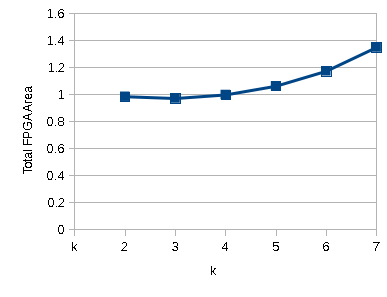
\includegraphics[scale=0.65]{k_vs_totalArea.png}
\caption{Total Area vs k}
\label{fig:Figure}
\end{subfigure}
\caption{Tradeoff in different k values}
\label{fig:Figure}
\end{figure}

We find that K=3 gives the least area estimates for implementing a given logic circuit on our FPGA. But we also observe that K=4 is also not bad and moreover is a power of 2 which makes it very attractive to divide large circuits into smaller circuits.



\section{CLB architecture: delay estimation}
\paragraph{}
Now, we move on to study the delay of implementing a given logic circuit on an FPGA of K-size CLBs. We first use the following equation derived in [3] to estimate the number of K-input LUTs required to implement an N-input design:
\begin{equation}
M_K = 2^{N-K}\cdot( 1 + \frac{1}{K} + \frac{1}{K^2} + ...) \approx 2^{N-K}\cdot\frac{1}{1-1/K}  
\end{equation}
And the depth of tree to implement N-input logic using K-input LUTs as derived in [3] is:
\begin{equation}
D_K = \frac{N-K}{x(K)}+1  
\end{equation}
where x(K) is the solution of:
\begin{equation}
K = x + 2^{x-1}  
\end{equation}
After dividing by technology dependent scaling factors, the dependence of $t_K$ (delay of implementing a given circuit on K-input LUTs) on k is shown in the Fig. Here, $\mu$ = $C_{R3}$/$C_{L3}$ increases with better technology nodes as routing capacitance starts becoming dominant compared to logic capacitance.

\begin{figure}[H]
\centering
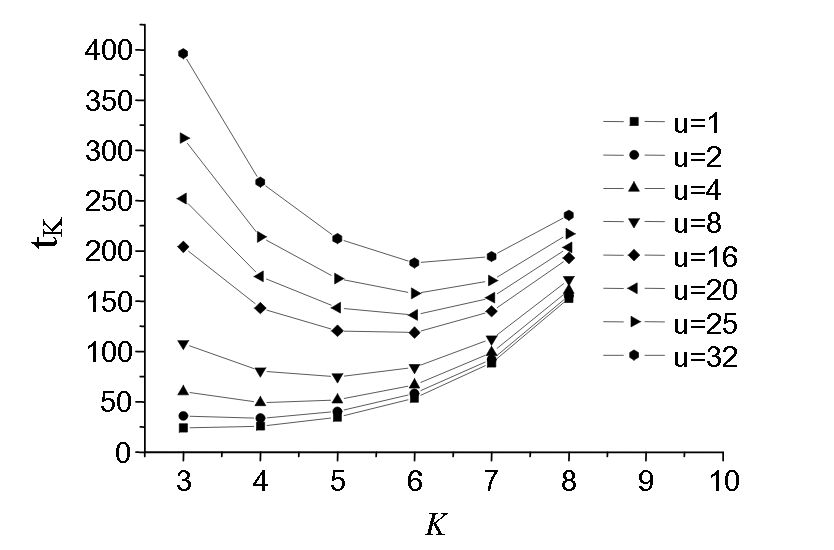
\includegraphics[width=\linewidth]{delay_vs_k.png}
\caption{$t_K$ vs k for different values of $\mu$}
\label{fig:Figure}
\end{figure}

For SCL 180nm technology node, we find a rough estimate of $\mu$ using schematic level captab analysis in Cadence ADE L to be $\mu$ = $20.5$/$8.25$ = $2.5$. As observed from the Fig., delay in case of K=3 is roughly 1.3 times the delay for K=4. This important observation dictates to select K=4 for optimal design in an Area-Delay Product sense. 
\section{CLB schematic}
\paragraph{}
The following schematic instances are used in the schematic of a CLB:

\begin{figure}[H]
\centering
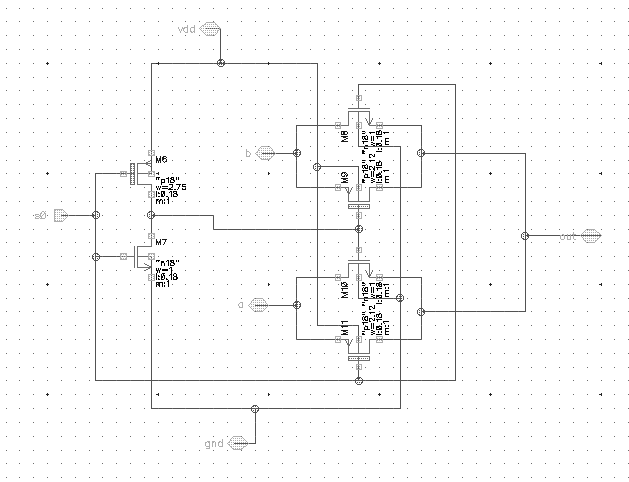
\includegraphics[scale=0.7]{2_1_mux.png}
\caption{2-to-1 MUX}
\label{fig:Figure}
\end{figure}
\begin{figure}[H]
\centering
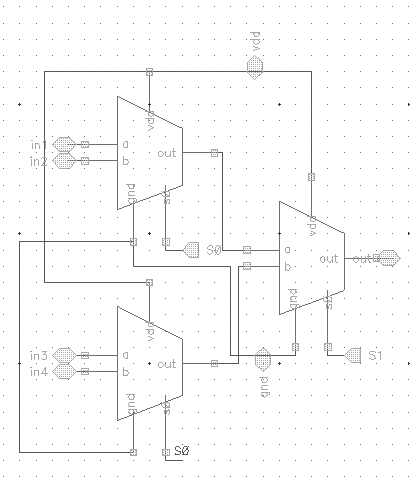
\includegraphics[scale=0.7]{4_1_mux.png}
\caption{4-to-1 MUX}
\label{fig:Figure}
\end{figure}
\begin{figure}[H]
\centering
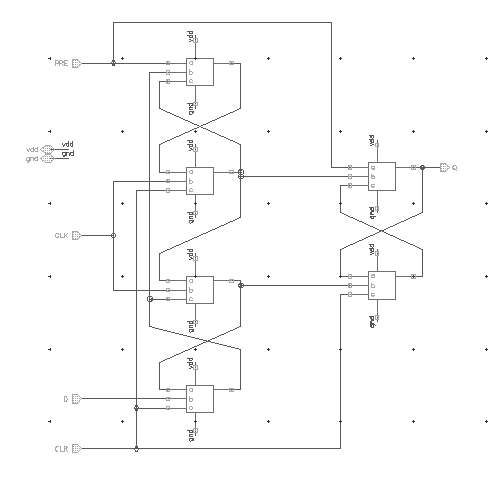
\includegraphics[scale=0.7]{DFF0.png}
\caption{D Flip-Flop}
\label{fig:Figure}
\end{figure}
\begin{figure}[H]
\centering
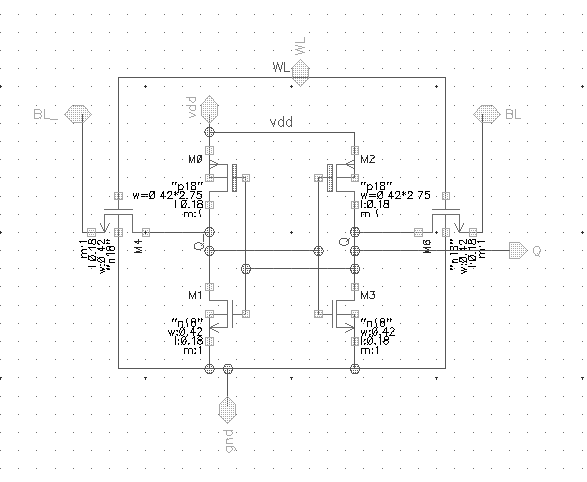
\includegraphics[scale=0.7]{sram_cell.png}
\caption{SRAM cell}
\label{fig:Figure}
\end{figure}
\begin{figure}[H]
\centering
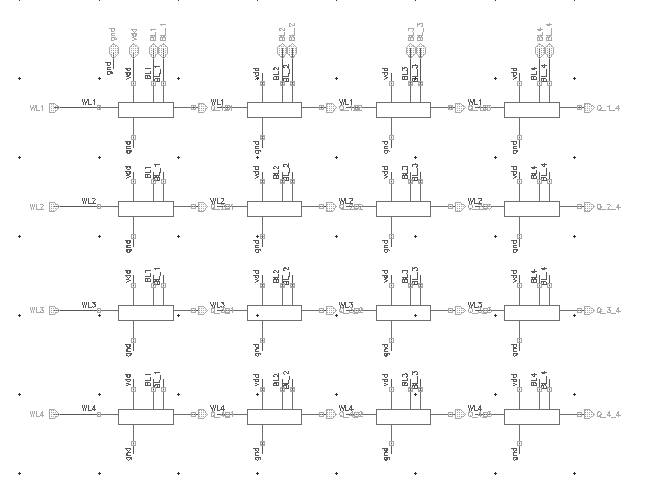
\includegraphics[scale=0.7]{sram_array.png}
\caption{4 X 4 SRAM array}
\label{fig:Figure}
\end{figure}
\begin{figure}[H]
\centering
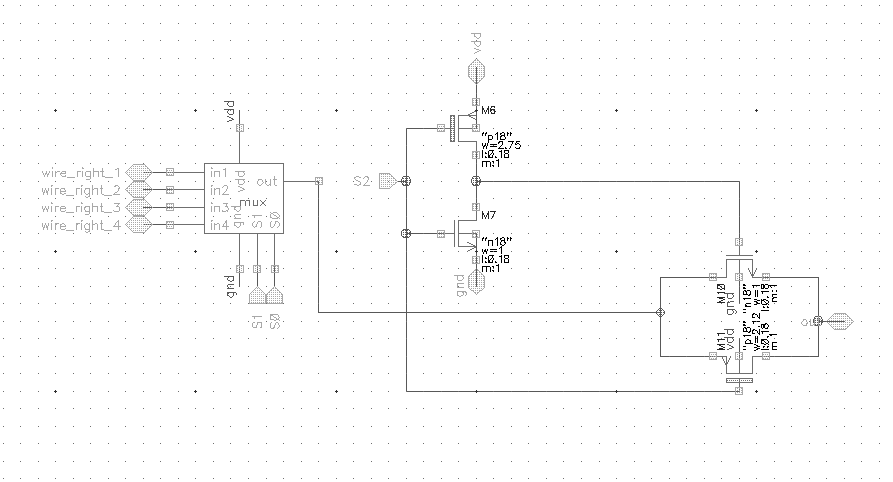
\includegraphics[scale=0.55]{4_1_crossbar.png}
\caption{4 X 1 Crossbar}
\label{fig:Figure}
\end{figure}
\begin{figure}[H]
\centering
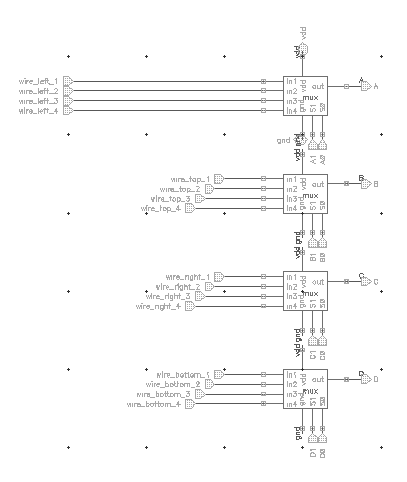
\includegraphics[scale=1]{4_4_crossbar.png}
\caption{4 X 4 Crossbar}
\label{fig:Figure}
\end{figure}


The components used in the schematic of CLB are described below:

\begin{itemize}
\item \textbf{4X4 LUT :} A 16 bit LUT arranged in a 4X4 6T-SRAM array to hold the truth table of a 4-input boolean function to be implemented. The Q-outputs of all the 16 SRAM cells are exposed. 
\item \textbf{4 X 1 Decoders :} A MUX tree of 5 4X1 decoder MUXes is formed to decode the 16 inputs to one output using 4 select lines.
\item \textbf{4X4 input crossbar :} A full crossbar to connect the 4 select lines to routing wires on left, right , top and bottom.
\item \textbf{4X1 output crossbar :} A full crossbar to connect the CLB output to one of the 4 routing wires on the CLB's right side.
\item \textbf{2X1 DFF MUX :} A mux to select whether to feed calculated boolean result in the DFF or retain its previous state.
\item \textbf{2X1 OUT MUX :} A mux to select whether to send the DFF value or the calculated boolean result out from the CLB.
\item \textbf{Inverter :} To invert the FF-initial-state
\item \textbf{NAND gates :} 2 NAND gates are used to form PRE and CLR signals for the DFF when config is HIGH
\item \textbf{D Flip-Flop :} Flip Flop provides 1-bit storage per CLB which can either be used to store current result of the LUT or to send out a previously stored value for further use in other parts of the FPGA.
\item \textbf{4X4 Configuration Memory :} A 16-bit SRAM arranged in a 4X4 6T-SRAM array to hold the configuration bits of the whole CLB. 
\begin{itemize}
\item 1-bit for FF-initial-state
\item 2-bits for the two MUXes
\item 8-bits for the 4X4 input crossbar
\item 3-bits for the 4X1 output crossbar
\item 2-bits left unused for future feature updates
\end{itemize}
\item \textbf{Bitlines :} 8 pairs of BL and ~BL go into each CLB for programming the two 4 X 4 arrays of SRAMs. The cells in the same column in an array share the same pair of bitlines.
\item \textbf{Wordlines :} 4 WL go into each CLB for programming the two 4 X 4 arrays of SRAMs. The row 1 of both 4 X 4 grids share the same WL and similar follows for other three rows.
\end{itemize}

\begin{figure}[H]
\centering
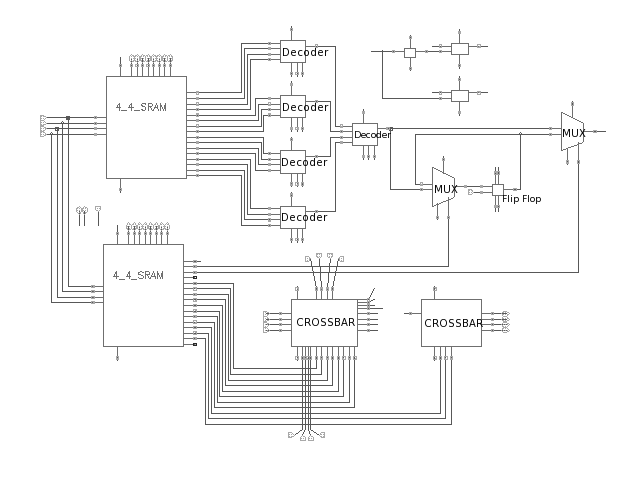
\includegraphics[width=\linewidth]{CLB_schematic.png}
\caption{CLB Schematic}
\label{fig:Figure}
\end{figure}




\section{Simulation Setup}
\paragraph{}

We are using Cadence Schematic L for designing the schematic and spectre is used in  Cadence ADE L to test the designs. SCL 180nm PDK has been used at tt\_18 configuration throughout the design. PMOS-to-NMOS ratio of 2.75 has been used at most places to get symmetric rise and fall characteristics with minimal sizing unless explicitly specified. This CLB is tested in ADE L using spectre for correct functionality.

\section{Summary}
\paragraph{}
This chapter presented the design of CLB along with the various derivations and modeling of area and delay to decide on an optimum LUT size in area-delay-product sense. We also decided on the total bits required for LUT and configuration.



